\subsection{Mandag \date{3. februar 2025}}

\paragraph{Von Neumann Stability Analysis}
\begin{itemize}
  \item Let \( U_m^n = \xi^n e^{i\beta m} \). Insert this into Difference Equation (DE).
  \item The method is Von Neumann Stable if \( \abs{\xi} \leq 1 + \mu K \) for all \( \beta \).
  \item Von Neumann stability is sufficient and necessary for pure IVP problems (Cauchy problems).
\end{itemize}
\begin{figure}[H]
  \centering
  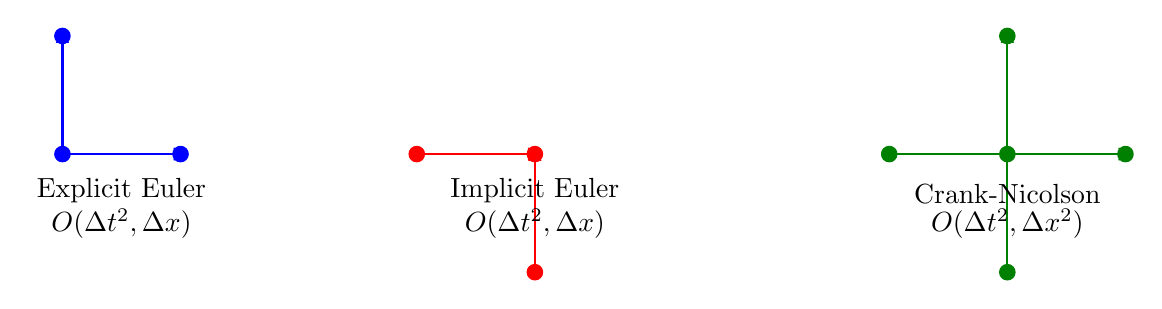
\begin{tikzpicture}[scale=1.5]
    % Explicit Euler (Forward)
    \begin{scope}[xshift=0cm]
      \fill[blue] (0,0) circle (2pt);
      \fill[blue] (0,1) circle (2pt);
      \fill[blue] (1,0) circle (2pt);
      \draw[->,thick,blue] (0,0) -- (1,0);
      \draw[->,thick,blue] (0,0) -- (0,1);
      \node[above] at (0.5,-0.5) {Explicit Euler};
      \node[above] at (0.5,-0.8) {$O(\Delta t^2, \Delta x)$};
    \end{scope}

    % Implicit Euler (Backward)
    \begin{scope}[xshift=4cm]
      \fill[red] (0,0) circle (2pt);
      \fill[red] (-1,0) circle (2pt);
      \fill[red] (0,-1) circle (2pt);
      \draw[->,thick,red] (-1,0) -- (0,0);
      \draw[->,thick,red] (0,-1) -- (0,0);
      \node[above] at (0,-0.5) {Implicit Euler};
      \node[above] at (0,-0.8) {$O(\Delta t^2, \Delta x)$};
    \end{scope}

    % Crank-Nicolson
    \begin{scope}[xshift=8cm]
      \fill[green!50!black] (0,0) circle (2pt);
      \fill[green!50!black] (1,0) circle (2pt);
      \fill[green!50!black] (-1,0) circle (2pt);
      \fill[green!50!black] (0,1) circle (2pt);
      \fill[green!50!black] (0,-1) circle (2pt);
      \draw[->,thick,green!50!black] (-1,0) -- (1,0);
      \draw[->,thick,green!50!black] (0,-1) -- (0,1);
      \node[above] at (0,-0.5) {Crank-Nicolson};
      \node[above] at (0,-0.8) {$O(\Delta t^2, \Delta x^2)$};
    \end{scope}
  \end{tikzpicture}
  \caption{Stencils for different numerical schemes}
  \label{fig:stencils}
\end{figure}



\begin{example}{Heat equation}{}
  \[
    u_t = u_{xx}, \quad 0 \leq x \leq 1, \quad 0 \leq t \leq 0.5
  \]
  \[
    \begin{cases}
      u(x, 0) = \sin(\pi x) \\
      u(0, t) = u(1, t) = 0
    \end{cases}
  \]
  \[
    u(x, t) = \sin(\pi x) e^{-\pi^2 t}
  \]

  \subparagraph{Finite Difference Scheme}
  \[
    \frac{1}{2k}\left( U_m^{n+1} - U_m^{n-1} \right) = \frac{1}{h^2}\left( U_{m-1}^n - 2U_m^n + U_{m+1}^n \right)
  \]

  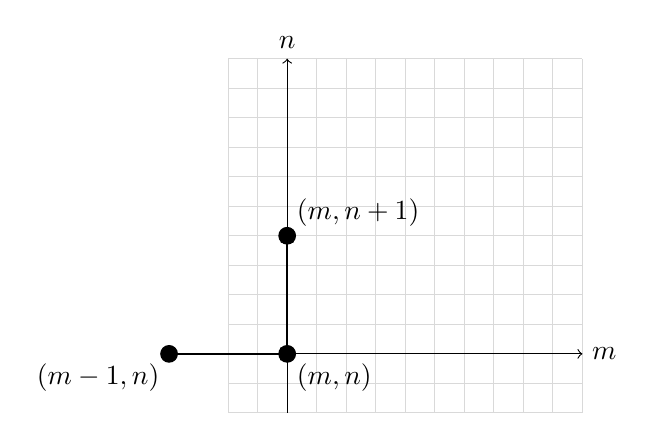
\begin{tikzpicture}[scale=1.5]
    % Grid
    \draw[step=0.25cm,gray!30] (-0.5,-0.5) grid (2.5,2.5);
    \draw[->] (-0.5,0) -- (2.5,0) node[right] {$m$};
    \draw[->] (0,-0.5) -- (0,2.5) node[above] {$n$};
    % Points
    \filldraw[black] (0,0) circle (2pt) node[below right] {$(m,n)$};
    \filldraw[black] (-1,0) circle (2pt) node[below left] {$(m-1,n)$};
    \filldraw[black] (0,1) circle (2pt) node[above right] {$(m,n+1)$};
    % Arrows
    \draw[->,thick] (0,0) -- (0,1);
    \draw[->,thick] (-1,0) -- (0,0);

  \end{tikzpicture}


  \subparagraph{Fourier Stability Analysis}

  \begin{align*}
    U_m^{n+1}
     & =
    2r\left( U_{m-1}^n - U_m^n + U_{m+1}^n \right) + U_m^{n-1}               \\
    \xi^{n+1} e^{i\beta x_m}
     & =
    2r\xi^n
    \left[
      e^{i\beta x_m - h} - 2e^{i\beta x_m} + e^{i\beta x_m + h}
      \right]
    + \xi^{n-1} e^{i\beta x_m}                                               \\
    \xi^2
     & =
    2r\left[ e^{-i\beta h} - 2 + e^{i\beta h} \right]\xi + 1                 \\
    \xi^2
     & =
    2r \left[ 2\cos(\beta h) - 2 \right]\xi+ 1                               \\
    \xi^2 + 8r\sin^2 \frac{\beta h}{2}\xi - 1
     & =
    0 \quad  \implies \quad \xi_\pm
    =
    -4r\sin^2 \frac{\beta h}{2} \pm \sqrt{16r^2\sin^4 \frac{\beta h}{2} + 1} \\
    \xi_- \leq - 1
    \quad
    \abs{\xi_-} \leq 1
  \end{align*}

  \textbf{Conclusion:} The scheme is unconditionally unstable.

  But we can stabilize the scheme by introducing a damping term (Du Fort-Frankel scheme):
  Replace \( U_m^n \leftarrow \frac{1}{2}(U_m^{n+1} + U_m^{n-1}) \) in the scheme.

  \begin{align*}
    \frac{1}{2k}\left( U_m^{n+1} - U_m^{n-1} \right)
     & =
    \frac{1}{h^2}\left( U_{m-1}^n + U_{m+1}^n\right) - \frac{1}{h^2}\left( U_m^{n+1} + U_m^{n-1} \right) \\
    (1 + 2r)U_m^{n+1}
     & =
    2r\left( U_{m-1}^n + U_{m+1}^n \right) + (1 - 2r)U_m^{n-1}                                           \\
    (1 + 2r)\xi^2 - 4r \cos \beta h \xi - (1 - 2r)
     & = 0                                                                                               \\
    \xi_\pm
     & = \frac{1}{1 + 2r} \left[ 2r\cos \beta h \pm \sqrt{4r^2\cos^2 \beta h + (1 - 2r)(1 + 2r)} \right] \\
    \xi_\pm
     & = \frac{1}{1 + 2r} \left[ 2r\cos \beta h \pm \sqrt{1 - 4r^2 \sin^2 {bh}} \right]                  \\
    \abs{\xi_\pm}^2 = \frac{2r - 1}{2r + 1} < 1 \quad \text{for all } r                                  \\
  \end{align*}

  \textbf{Conclusion:} The method scheme is unconditionally stable, for all \( r \).

  Now we know that the scheme has stability for all \( r \), it might still not converge because we also need consistency.

  \subparagraph{Consistency}
  \begin{align*}
    \tau_m^n
     & =
     & \frac{1}{2k}\left( u_m^{n+1} - u_m^{n-1} \right)                                                 \\
     & - \frac{1}{h^2}\left( u_{m-1}^n - u_{m+1}^n \right)                                              \\
     & + \frac{1}{h^2}\left( u_m^{n+1} - u_m^{n-1} \right)                                              \\
     & =
     & \frac{1}{2k}\left[ 2k u_t + 2k^3 \frac{1}{3!}u_{tt} + \ldots \right]                             \\
     & -\frac{1}{h^2}\left[ 2u + 2h^2 \frac{1}{2!}u_{xx} + 2h^4 \frac{1}{4!}u_{xxxx} + \ldots \right]   \\
     & + \frac{1}{h^2}\left[ 2 u + 2k^2 \frac{1}{2!}u_{tt} + 2k^4 \frac{1}{4!}u_{tttt} + \ldots \right] \\
     & =
    u_t - u_xx 
    + \frac{k^2}{h^2}u_{tt} + \frac{k^2}{3!}u_{tt} 
    + \frac{h^2}{12}u_{xxxx} + \frac{k^4}{12h^2}u_{tttt} 
    + \ldots
  \end{align*}
  The method is consistent only if the truncation error goes to zero as \( h, k \to 0 \).

  Here the method is consistent when \(\frac{k}{h} \underset{h,k \to 0}{\longrightarrow} 0\).

  \textbf{Conclusion:} The method is conditionally consistent.

  \textbf{Conclusion:} The method is conditionally stable and consistent for all \( r \) and \( \frac{k}{h} \underset{h,k \to 0}{\longrightarrow} 0 \) and therefore convergent.

\end{example}

\subsection*{Domain of dependence}



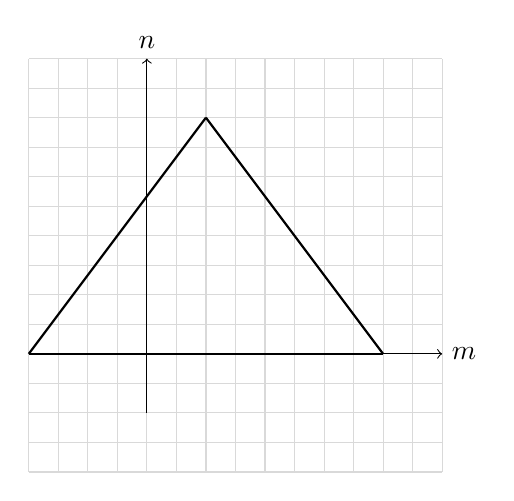
\begin{tikzpicture}[scale=1.5]
  % Grid
  \draw[step=0.25cm,gray!30] (-1,-1) grid (2.5,2.5);
  \draw[->] (-1,0) -- (2.5,0) node[right] {$m$};
  \draw[->] (0,-0.5) -- (0,2.5) node[above] {$n$};

  % Triangle
  \draw[-,thick] (-1,0) -- (0.5,2);
  \draw[-,thick] (-1,0) -- (2,0);
  \draw[-,thick] (2,0) -- (0.5,2);

\end{tikzpicture}


